% Basic LaTeX template for NE 204 lab report
\documentclass[11pt]{article}

%==============================================================================
%%% Everything between the "="'s is the preamble.
%%% Define packages and meta data here

% Common packages
\usepackage{amsmath}    % Expanded math
\usepackage{amssymb}    % Expanded math symbols
\usepackage{graphicx}   % For images
%\usepackage[version=3]{mhchem} % For nuclide formatting

% All images/figures will be stored in the images folder.
% Specify that here so pdflatex knows where to look for images.
\graphicspath{{./images/}}

% Metadata
\title{Lab 0 Report}
\author{Darrell Stepter}
\date{\today}
%==============================================================================

\begin{document}

% Compile metadata from preamble into a nicely-rendered title section
\maketitle

% The *'s next so section/subsection definitions suppresses numbering
\section*{Introduction}
\label{sec:intro}
Introduction / motivation / background go here.


\section*{Methods}
\label{sec:meth}
Experimental procedure / set up / methods go here.

2. Discuss the approach to the energy calibration (N.B. there is no experimental setup" in this case).


\section*{Results}
\label{sec:res}
Experimental results go here.

3. Present the results of your energy calibration and include any relevant discussion.

%\begin{figure}[h!]
%  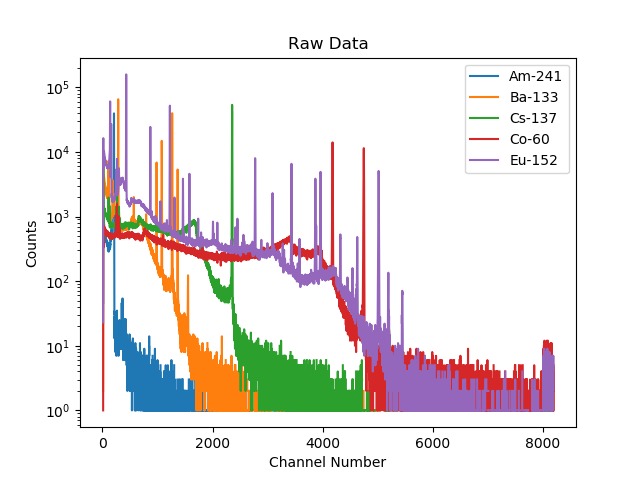
\includegraphics[width=\linewidth]{Raw_Spec.png}
%  \caption{Raw Spectrum Data.}
%  \label{fig:Raw_Spec1}
%\end{figure}

%Figure \ref{fig:Raw_Spec1} shows the uncalibrated raw spectrum data.


%\begin{figure}[h!]
%  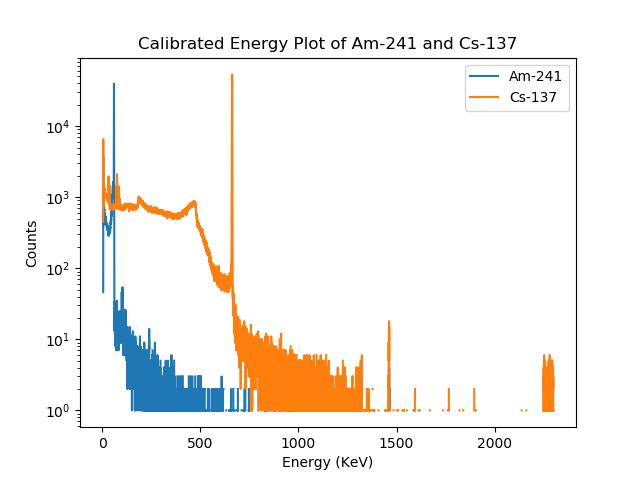
\includegraphics[width=\linewidth]{Cal_AmCs_Spec.png}
%  \caption{Calibrated Americium and Cesium Spectrum.}
%  \label{fig:Cal_AmCs_Spec1}
%\end{figure}

%Figure \ref{fig:Cal_AmCs_Spec1} shows the calibrated spectrum data for Am-241 and Cs-137.

\begin{figure}[h!]
%  \centering
  \begin{subfigure}[b]{0.6\linewidth}
    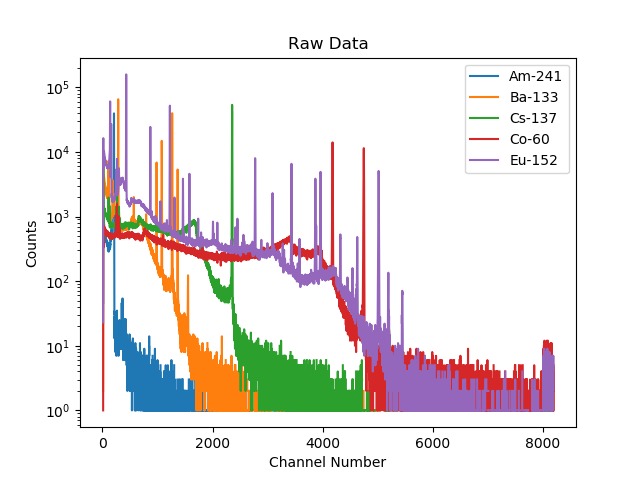
\includegraphics[width=\linewidth]{Raw_Spec.png}
    \caption{Raw Spectrum Data.}
  \end{subfigure}
  \begin{subfigure}[b]{0.6\linewidth}
    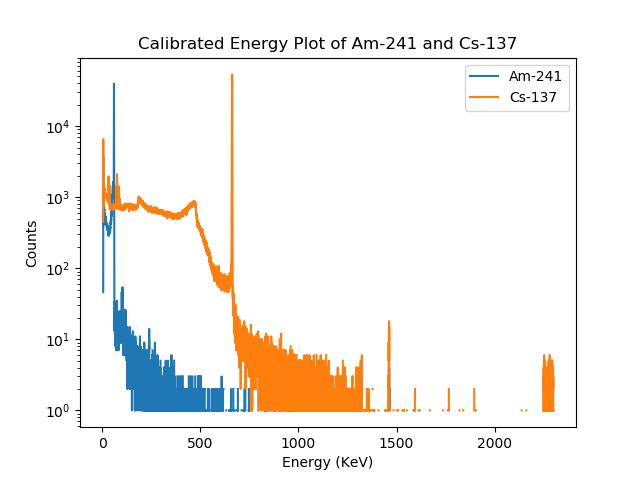
\includegraphics[width=\linewidth]{Cal_AmCs_Spec.png}
    \caption{Calibrated Am-241 and Cs-137 Spectra.}
  \end{subfigure}
  \caption{Raw data and Calibrated Spectra.}

\end{figure}

\csvautotabular{/Users/darrellstepter/repos/school/NE204/Lab0/dvstepter-lab0/images/peakdiffquant.csv}


\section*{Discussion}
\label{sec:disc}
Discussion of results / limitations / conclusions go here.


% Bibliography
\bibliographystyle{plain}
% Refers to a bibtex file in the current dir named "references.bib"
\bibliography{references}

\end{document}
